\chapter{Performance Evaluation}
\label{cha:evaluation}

Answering the question of the GC performance under a real-world setting,
this chapter discusses the performance evaluation I undertook for analyzing
the Garbage-First family of garbage collectors. This chapter will firstly describe the software and hardware platform I used for benchmarking,
Then the detailed evaluation process and results of both pause time and
barrier latency will be presented and discussed.

Section~\ref{sec:dacapo} and \ref{sec:hardware} roughly introduce the experimental
platform and software involved for the performance measurements.
Section~\ref{sec:generalmethod} discusses the generall evaluation method used to
evaluate the performance of all the interested metrics.
Section~\ref{sec:pausetime}, \ref{sec:barrierlatency} and \ref{sec:remsetsize} discusses the detailed
measurement steps involved to evaluate the GC pause time, barrier overhead and remembered set size
respectively, as well
as figures of the results and the discussion based on the results.

\section{The Dacapo Benchmark} % 2
\label{sec:dacapo}

The Dacapo Benchmark Suite is a tool for Java benchmarking and contains a set of
open-sourced real-world programs with a high memory load.

The Dacapo Benchmark is frequently used during the development of the G1 family
of garbage collectors in chapter~\ref{cha:implementation}, as a validation program
to verify the correctness of the collectors under a real-world setting.

I also performed pause time evacuations and barrier latency evaluation
on all of the following Dacapo Benchmark suites.
The benchmarking suites I used for evaluation includes (\cite{Blackburn:2006:DBJ:1167515.1167488}):

\begin{itemize}
  \item \textbf{luindex} Uses lucene to indexes a set of documents; the works of Shakespeare and the King James Bible
  \item \textbf{bloat} Performs a number of optimizations and analysis on Java bytecode files
  \item \textbf{hsqldb} Executes a JDBCbench-like in-memory benchmark, executing a number of transactions against a model of a banking application
  \item \textbf{lusearch} Uses lucene to do a text search of keywords over a corpus of data comprising the works of Shakespeare and the King James Bible
  \item \textbf{pmd} Analyzes a set of Java classes for a range of source code problems
  \item \textbf{xalan} Transforms XML documents into HTML
  \item \textbf{avrora} Simulates a number of programs run on a grid of AVR microcontrollers
  \item \textbf{sunflow} Renders a set of images using ray tracing
\end{itemize}

By performing evaluations on a wide range of benchmarking suites which represents different
classes of real-world programs, it is more possible to understand the pros and cons
of the G1 family of collectors under a real-world setting.

\section{Hardware Platform} % 2
\label{sec:hardware}

During the implementation of all the G1 family of garbage collectors in chapter~\ref{cha:implementation},
a list of machines with a large variety on CPU types, clock, number of processors and
the size of cache and memory were involved, as shown in Table~\ref{tab:machines}.
By executing all the benchmarking suite of the Dacapo Benchmark on these different machines,
and thanks to the benchmarking suites of the Dacapo Benchmark which reflect
different categories of programs in the real world,
we have the ability to statistically verify the correctness of the previously
implemented garbage collectors (in chapter~\ref{cha:implementation})
and make sure they perform as intended in a real-world setting.

For further performance evaluation, the "fisher" machine was used for the final benchmarking.

\begin{table*}
  \centering
  \input table/machines.tex
  \caption{Machines used for development and evaluation.}
  \label{tab:machines}
\end{table*}

\section{General Measurement Methodology}
\label{sec:generalmethod}

I perform both GC pause time and barrier overhead measurements on the optimized build
of the JikesRVM, with 6 different GC configurations for the 6 GCs to be measured respectively.
To collect measurement results, I execute all 10 DaCapo benchmark suites discussed in section~\ref{sec:dacapo}
on all 6 collectors, with respect to 4 different heap sizes, 637\,MB, 939\,MB, 1414\,MB, and 1971\,MB
respectively. Each benchmark suite is executed 10 times for each configuration of $(GC, HeapSize)$ to
collect more precise results and avoids the error due to some unexpected environmental fluctuations.

\subsection{Reducing non-determinisms}
\label{subsec:nondeterminisms}

The adaptive compiler can have non-deterministic behaviors when performing dynamic
compilations and optimizations to the executing Java program. In order to minimize
such non-deterministic behaviors and makes the program executes more faster, I performed
the measurement methodology called "warmup replay", which was firstly introduced by
\cite{yang2012barriers}, as a replacement of the "pseudoadaptive approach" introduced by \cite{blackburn2004barriers}.

This methodology performs an execution of 10 iterations for each benchmark suite to
collect runtime execution information before the measurement, to assist with more optimized compilation.
Then during measurements, after the first iteration of warmups, JikesRVM compiles all
methods by using the advice information generated previously to avoid any re-compiling
behaviors during the following measurement iteration.

I ran all of the 9 benchmark suites discussed in section~\ref{sec:dacapo} on each collector
for 10 times, with 2 times of warmup execution before the timing iteration.
JikesRVM performs warmup-replay compilation at the end of the first warmup iteration.

\section{Pause Time Evaluation} % 7
\label{sec:pausetime}

This section describes the steps took for pause time evaluation as well as
all the evaluation results and discussions.

\subsection{Mutator latency timer}

In order to perform more careful analysis on the mutator pause times, instead of
simply calculating the time starting from the first stop-the-world phase to the last
stop-the-world phase during each GC cycle, I implemented a mutator latency timer
to perform a more precise calculation of mutator pause times.

The mutator latency timer contains a static "three-dimensional" array:\\
\centerline{\textjava{static long[] LOGS = long[THREAD ID * EVENT ID * NUM_LOGS]}}
This array is statically allocated within the VM Space to record the timestamp (in nanoseconds)
of each event, for each mutator. The first dimension is the thread id of all
mutators. The second dimension is the event id. The third dimensional \textjava{NUM_LOGS} is the
max number of logs of one thread and is currently set to $1024$. Particularly under
the current context, to measure the pause time for each mutator, two events,
\textjava{MUTATOR_PAUSE} and \textjava{MUTATOR_RESUME} are defined to record the time when a
mutator thread starts waiting for GC complete and the time when a mutator gets resumed for execution.

In JikesRVM, a mutator thread checks for GC requests and starts waiting if necessary every
time it reaches a yieldpoint, which may trigger a \textjava{MUTATOR_PAUSE} event if it should
be paused. After a stop-the-world cycle is finished, before continuing for further execution,
it triggers a \textjava{MUTATOR_RESUME} event.

At the end of the benchmark execution, the mutator latency timer will dump all the
data in the \textjava{LOGS} array to the print buffer for further data analysis.

As an output of the analysis of the overhead data, I report the minimum, 25\%, 50\%,
75\% and maximum mutator pause time for each GC, each benchmark suite and each heap size.

\subsection{MMTk harness callbacks}

During each iteration of benchmarking, the Dacapo benchmark has several warm-up
executions which will run the benchmark suite a few times to warm up the cache and JVM.
Then the DaCapo benchmark will start the actual benchmarking run. I use a probe called \textjava{MMTKCallback}
which will call the \textjava{org.mmtk.plan.Plan.harnessBegin} method
before the final benchmarking execution and call the \textjava{org.mmtk.plan.Plan.harnessEnd}
after the final benchmarking execution. Based on this, the two callbacks
\textjava{harnessBegin} and \textjava{harnessEnd} are used to calculate the inform the mutator
latency timer to start recording logs or dump all logs.

\subsection{Results}

\begin{table*}
  \centering
  \label{tab:pause}
  \input table/average-pause.tex
  \caption{Results of the GC pause time}
\end{table*}

\begin{figure*}
  \centering
  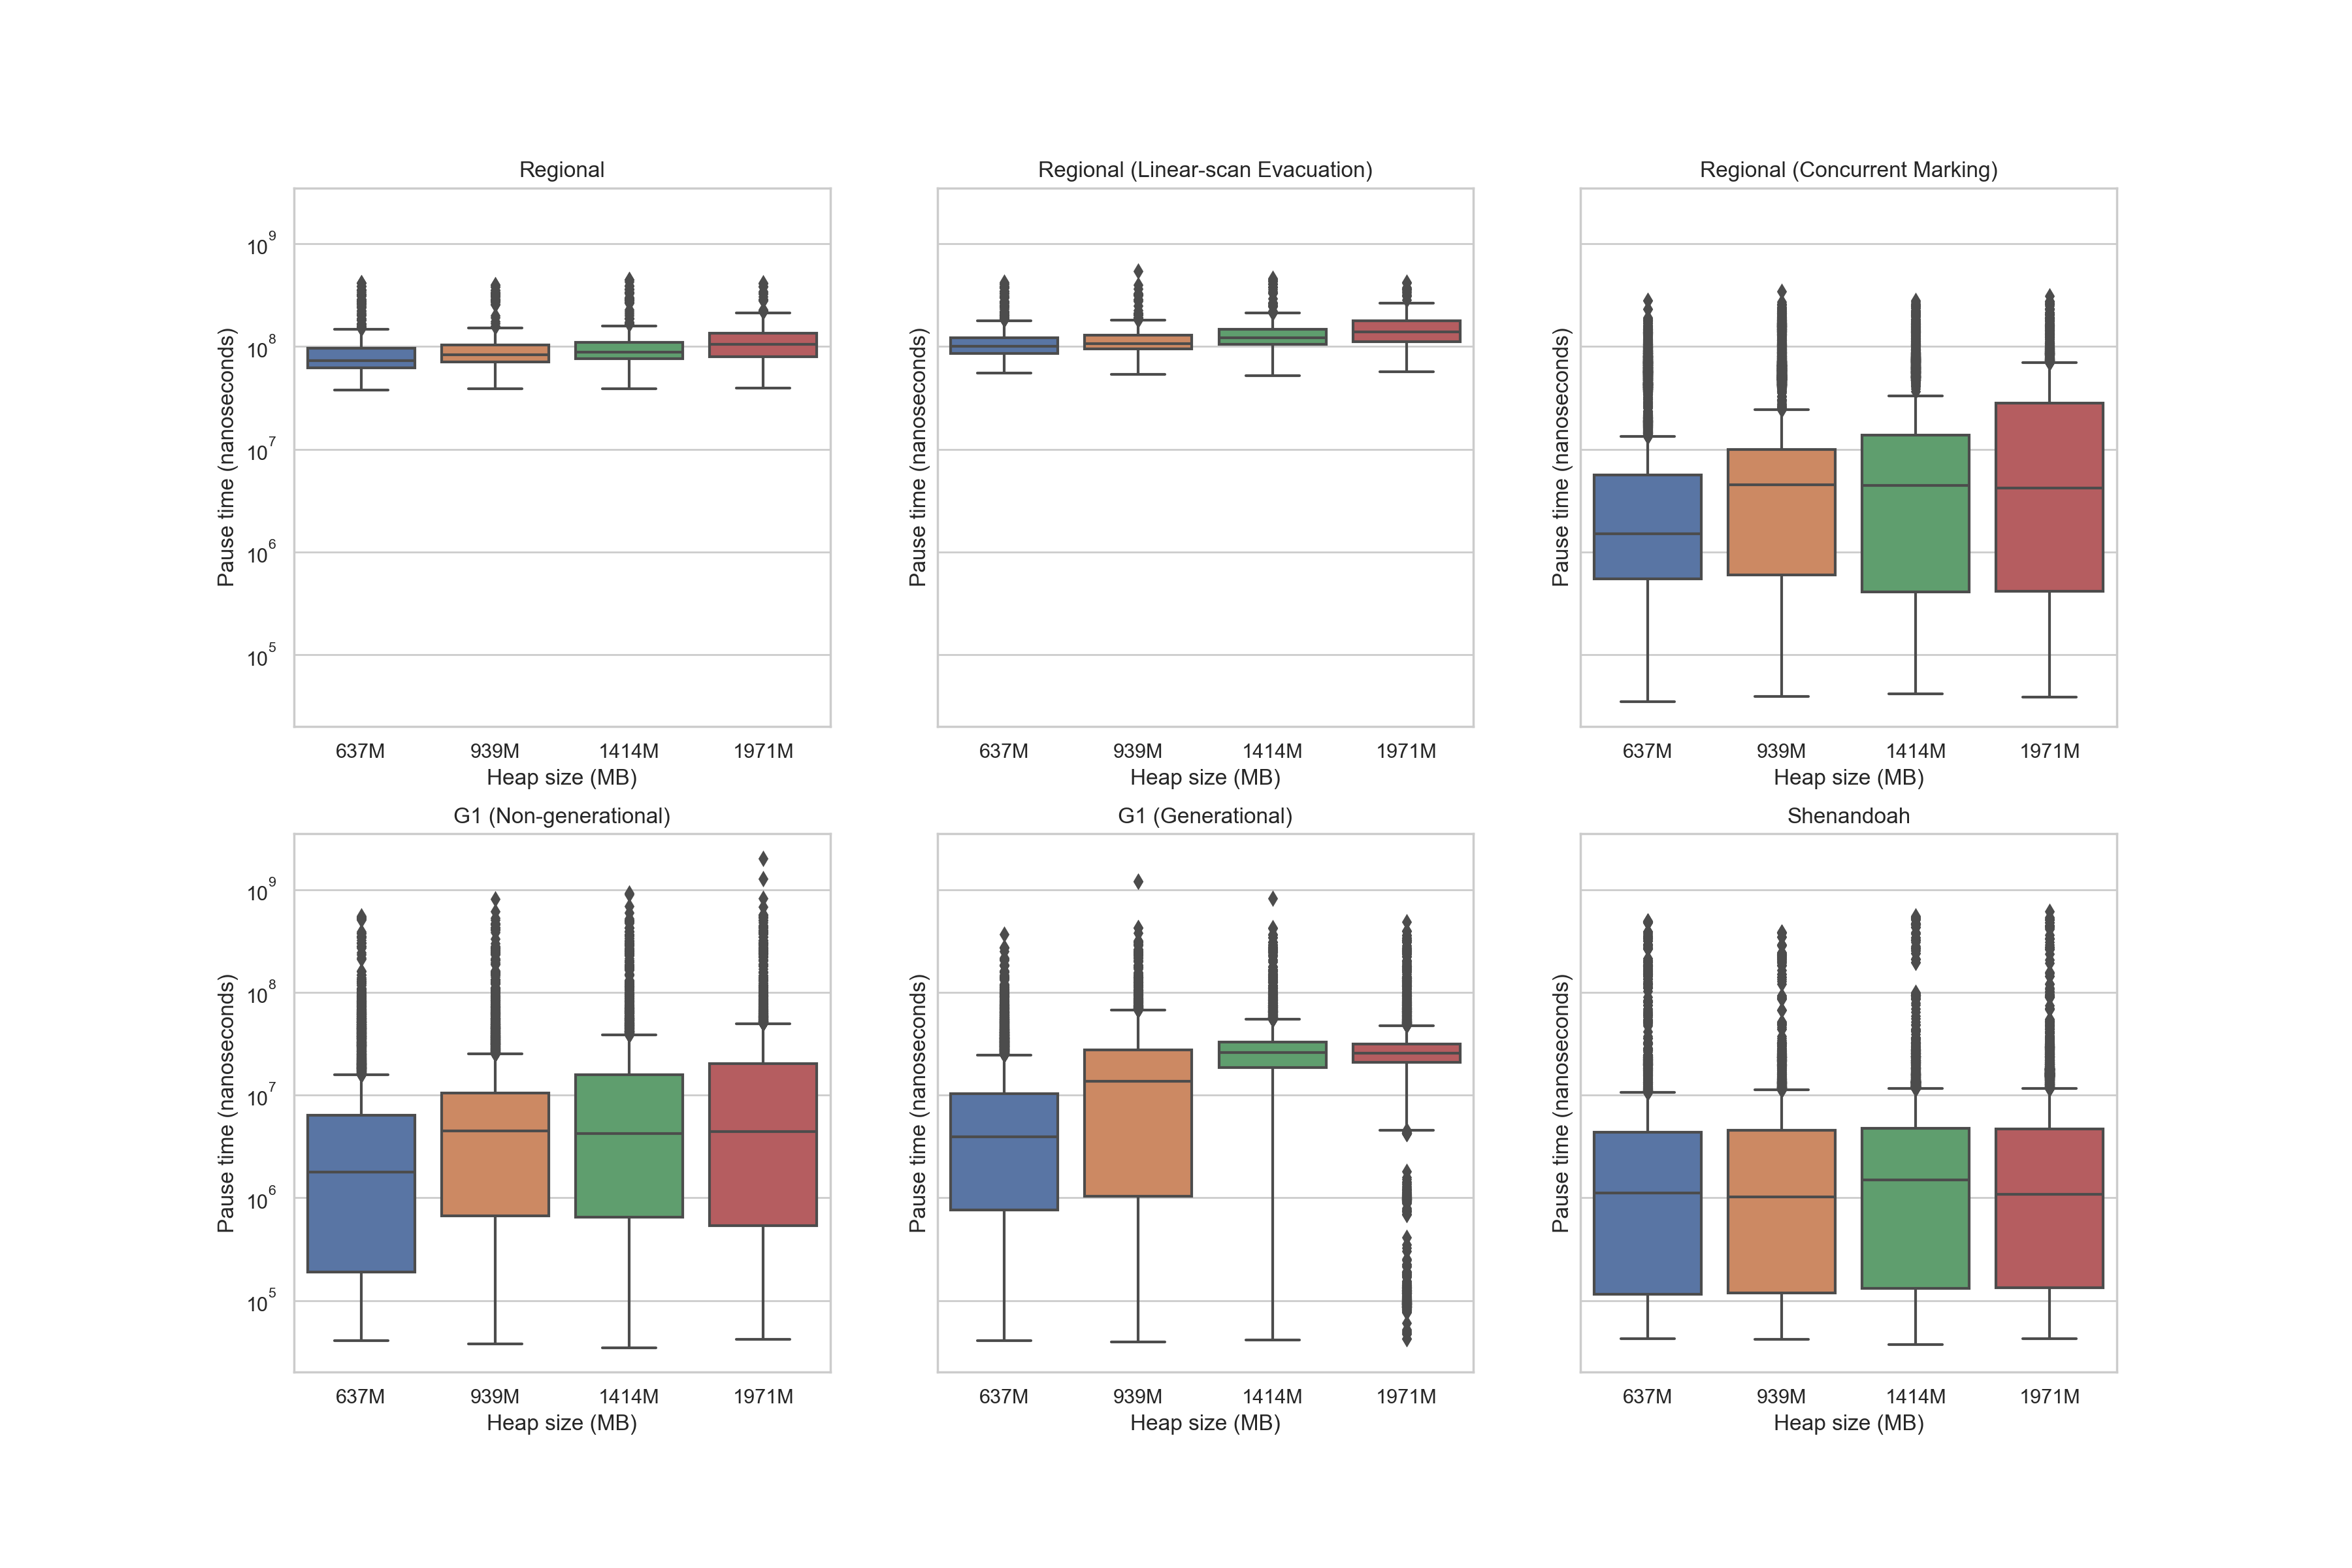
\includegraphics[width=\textwidth/1]{{figs/pause-time.png}}
  \caption{Pause times of 6 collectors}
  \label{fig:pausetime}
\end{figure*}

\begin{table*}
  \centering
  \input table/full-gc-ratio.tex
  \caption{Ratio of full gc}
  \label{tab:fullgc}
\end{table*}

Figure~\ref{fig:pausetime} shows the results of the GC latency time
evaluated on all 6 garbage collectors discussed in section~\ref{cha:implementation}.
Each subfigure shows
the overall GC latency time for each garbage collector. Specifically, the
minimum, 25\% percentile, medium, 75\% percentile and maximum GC latency time nanoseconds
were reported for each collector and each heap size.

To present the results more clearly, the benchmarking results are presented as
a set of box plots and with log-scaled pause time y in nanoseconds as the y-axis.

\subsection{Discussion}

As the most simple form of the G1 family of GC, the Regional collector, performs fully
stop-the-world GC during each GC cycle. Works for each GC cycle includes marking all
live objects and walk over the object graph to evacuate objects in a set of selected memory
regions. Totally 2 full heap tracings are performed during each GC cycle, which makes the GC
pause time longer. The average pause time for this Regional GC generally ranges from $104$ to $147$
milliseconds and increases as the heap size increases.

By performing linear scan based evacuation, the linear-scan evacuation version of the Regional
GC has to scan the memory regions in the collection set twice, one for exacuating live objects and
one for updating references. In this way, the collector generally has longer pause times,
which ranges from $139$ to $198$ milliseconds in average and increases as the heap size increases.
The percentage of GC pause time increase are 33.7\%, 30.5\%, 26.9\%, 34.8\% for 4 heap sizes
respectively, in average 31.5\%.
Although performing linear scan evacuation can largely increase the GC pause time,
this independent phase is an important part for G1 GC and the Shenandoah GC.

After performing concurrent marking in addition to the linear scan based evacuation,
the resulting ConcRegional collector split the pause for marking into several smaller
pauses and performs most of the marking work in concurrent without stopping the mutators.
This makes the total pause time for a GC smaller and significantly reduces the average
pause time by 88.5\%.

The non-generational G1 reduces the collection size to meet a pause time goal of 100\,ms.
Based on the benchmarking results, at least 75\% of the pauses are less than the pre-defined
pause time goal. On the other hand, G1 uses remembered sets to update references
instead of performing full heap tracing.
To small heaps this has almost no benefits, even increases the average pause time by
16.2\% on 637\,MB heaps. But for heap sizes of 39\,MB, 1414\,MB, and 1971\,MB, this
partial heap scanning technique reduces average pause time by 8.8\%, 7.4\% and 10.7\%
respectively. So the remembered sets based references updating has more benefits on
larger heaps. However, the full GC becomes more expensive because of the large work required
to update all the remembered sets in the heap, which usually results in a pause time
ranges from 0.5\,s to 1.5\,s.

By using the generational G1 GC, young/nursery GCs are usually triggered several times
before a major GC happens. Also, nursery GCs are fully stop-the-world and always tries
to collect as much nursery regions as possible, as long as the pause time does not exceed
the pre-defined pause time goal. This results in the increase of GC pause times.
However, the generational collection can largely reduce the probability of G1 GC falling
back to full GCs. As shown in Table~\ref{tab:fullgc}, I measured the overall full GC ratio
for both non-generational and generational G1 GC on four different heap sizes,
with a 95\% confidence interval reported as well.
Based on the results, with the generational mode, G1 reduces the
probability of falling back to full GC by 12.5\%.

The Shenandoah GC performs marking, evacuation and reference updating in concurrent,
this significantly reduces the pause time by 72.6\%, compared to the concurrent marking version
of the regional collector. Based on the benchmarking results at least 75\% of
the GC pauses do not exceed 10 milliseconds. However, full GCs can still result
in pauses of around 500 to 600 milliseconds, which is longer than the concurrent-marking
regional collector due to the Brooks barrier involved during the evacuation phase, which performance
will be discussed in section~\ref{sec:barrierlatency}

\section{Barrier Latency Evaluation} % 7
\label{sec:barrierlatency}

This section describes the steps took for barrier overhead evaluation as well as
all the evaluation results and discussions.

\subsection{Methodology}

The mutator barrier percentage overhead is modeled as follows:
$$
\text{Overhead} = \frac{|\text{Mutator time with barrier} - \text{Mutator time without barrier}|}{\text{Mutator time without barrier}} * 100\%
$$

The mutator execution time is calculated as the execution time of the benchmarking program with
stop-the-world GC time excluded.

As discussed in chapter~\ref{cha:implementation}, I implemented the Garbage-first
family of collectors by performing progressive improvements on a simple region-based collector.
In this way, after performing an algorithmic improvement on a collector, we can measure the overhead of
the newly involved barriers or other technologies by comparing the benchmarking results
of the old collector and the new collector.

As an output of the analysis of the overhead data, the average barrier overhead
for each GC, each benchmark suite, each heap size and each barrier this project used is reported
as well as their corresponding 95\% confidence interval.
The overall average overhead and its 95\% confidence interval for each barrier are also reported.

\subsection{Snapshot-at-the-beginning barriers}

\begin{table*}
  \centering
  \input table/satb-barrier.tex
  \caption{Snapshot-at-the-beginning barrier overhead}
  \label{tab:satbbarrier}
\end{table*}

Table~\ref{tab:satbbarrier} shows the overheads of the Snapshot-at-the-beginning barrier
as well as their 95\% confidence interval on different heap sizes. Based on the evaluation data, the SATB barrier used for concurrent-marking
has an overhead of 22\% on average.

As a deletion barrier, during concurrent marking, the barrier will trace and mark
all deleted nodes (i.e. the old object field when performing assignment \textjava{obj.x = y}) in the object graph.
A major difference between the SATB barrier used in these region-based collectors and
the concurrent mark-sweep GC is that the concurrent mark-sweep GC only marks objects
when tracing an object (the mark data is usually stored in the object header).
But the currently implemented G1 family of collectors have to count the live bytes
for each region to assist with further collection set selection.
Also, these G1 family of collectors uses off-heap mark table instead of object header to store
mark data. For these reasons, a lot of atomic operations should be done during concurrent
marking which further reduces the mutator throughput, compared to the concurrent mark-sweep GC.
% The data shows that the SATB barrier increases the average mutator overhead by 92.93\%,
% which is an unignorable overhead. As a significant reason for causing such large overhead,
% all region-based

\subsection{Remembered set barriers}

\begin{table*}
  \centering
  \input table/remset-barrier.tex
  \caption{Remembered set barrier overhead}
  \label{tab:remsetbarrier}
\end{table*}

Table~\ref{tab:remsetbarrier} shows the overheads of the Remembered set barrier
as well as their 95\% confidence interval on different heap sizes.

This result represents the mutator overhead of both remembered-set barriers and concurrent remset refinements.
The design of the remembered-set barriers and the remset refining process follows
the original design of G1 where only 1 thread is used to process the dirty card
buffer and it only awakes for processing when the card buffer is full.

Based on the measurement results, the overhead of remembered-set barriers is not low,
which is 59.65\% on average. This is because the number of threads used for remset refinement
is not enough and the dirty card buffer always becomes full. Under such situation,
mutators have to take part of the responsibility to process cards in their local buffer,
which significantly reduces its throughput.

A possible fix, which is already be introduced into the OpenJDK's G1 implementation, is
to spawn more threads for remset refinement, and refinement threads can start processing cards earlier,
not necessarily need to wait until the global card buffer is full.

\subsection{Brooks indirection pointer barriers}

\begin{table*}
  \centering
  \input table/brooks-barrier.tex
  \caption{Brooks indirection pointer barrier overhead}
  \label{tab:brooksbarrier}
\end{table*}

Table~\ref{tab:brooksbarrier} shows the overheads of the Brooks indirection pointer barrier
as well as their 95\% confidence interval on different heap sizes.
On average, by using the Brooks indirection barrier, the mutator overhead
is increased by 85.46\%.

This is a significant high overhead. The reason for causing this is the use of 
"use barriers" which insert a barrier every time the JVM wants to access and use
an object reference. In addition, during the concurrent evacuation phase,
an extra barrier is used for every the object comparison operation
to ensure the correct comparison between the forwarded and unforwarded pointer of the same object reference,
which further increases the mutator overhead.

However, in order to perform concurrent evacuation and reference updating, the handling
of forwarded and unforwarded pointers is necessary.
One possible improvement is to use "colored pointers" to ensure the CPU will always access
the new version of the object pointer before using this pointer,
instead of go through the indirection pointer every time the mutator access the object.

\pending{A figure to explain the 'Use barrier'}

\section{Remembered-Set Size} % 7
\label{sec:remsetsize}

As part of the evacuation of the G1 collector, I measured the remembered-set footprint
of G1 GC.

The implementation of remembered-set follows the design of the original OpenJDK
implementation, which uses a list of \textjava{PerRegionTable} as remembered-set
for each region. Each \textjava{PerRegionTable} remembers cards in one foreign region.
\textjava{PerRegionTable} is implemented as a bit table where each bit corresponds
to a card in the corresponding foreign region. 

Under such implementation, theoretically the space complexity for remembered-sets
is $O(N^3)$ where $N$ is the number of regions in the heap. Because every region
has its own remembered-set and each remembered-set consists of $N-1$ \textjava{PerRegionTable}s
to remember cards in other $N-1$ regions. However, the practical space performance
of such remembered-set structure has never been formally measured.

Due to the same remembered-set structure,
measurements for the remembered-set footprint of JikesRVM's G1 implementation can reflect
the footprint of the OpenJDK's implementation, which can help us understand the
space performance of G1's remembered-sets under a real-world setting.

\subsection{Evaluation metrics}

In order to measure the remembered-set footprint carefully, two metrics are proposed
to reflect the space performance of remembered-sets:

\textbf{Committed Memory Ratio} is the ratio of the memory allocated for building remembered-sets
versus the total committed memory at some specific execution point.
This metric reflects the proportion of the heap that remembered-sets are actually take up.

$$ \text{Committed Memory Ratio} = \frac{\text{Committed memory for remset}}{\text{Total committed memory}} $$

\textbf{Utilization Ratio} is the ratio of the memory (in bits) actually used for
remembered-sets to remember the cards, versus the total memory allocated for remembered-sets.
This metric reflects the proportion of the remembered-sets that is actually in use
and not be wasted.

$$ \text{Utilization Ratio} = \frac{\text{Bits actually used for store cards}}{\text{Committed memory for remset in Bits}} $$

\subsection{Results \& discussion}

Remembered-set size is always changing during the execution of the program.
Plus, as the remembered-set refinement thread may still processing cards,
the remembered-set can be incomplete due to in such situation some cards are still waiting to
be processed and write to some remembered-sets.

For this reason, I measure the remembered-set footprint at the start of each GC pause, immediately after
the stop-the-world remembered-set refinement is finished. At this time the remembered-set
footprint reaches a steady state, the remembered-set is complete and contains
all the corresponding cards under current heap state.

\begin{table*}
  \centering
  \input table/remset-size.tex
  \caption{Remembered set footprint}
  \label{tab:remsetfootprint}
\end{table*}

As shown in Table~\ref{tab:remsetfootprint}, I measured both proposed metrics
on both non-generational and generational G1 GC, with four different heap sizes.
For each mode of G1 GC and each heap size, I report the minimum value, maximum value and mean value
with 95\% confidence interval for both committed memory ratio and utilization ratio.

Based on the footprint data, we can see that on average 9.0\% of the comment memory
is allocated for building remembered-sets, with a maximum proportion of 38.2\%.
Which means remembered-sets are taking up too much memory in the heap. 
Also, the memory usage (i.e. utilization) for remembered-sets is pretty low,
only 8.2\% of the memory allocated for remembered-sets is actually used for remembering cards.
Taking the high committed memory ratio into consideration, this means that the
space efficiency of the \textjava{PerRegionTable} based remembered-sets is extremely
low. Hence a lot of optimization works should be done to further reduce the memory
waste of remembered-sets.

\section{Summary} % 2
\label{sec:summary}

This chapter discusses the measurement methodology and results for evaluating the
performance of the G1 family of garbage collectors. This includes the evaluation of
GC pause times and overhead of several mutator barriers. Also, the phenomenon revealed
in the measurement results is carefully discussed.

On the one hand, based on the measurement results, we can see that linear scan based evacuation
increases the work for each GC. Using concurrent marking, concurrent evacuation
or remembered set based partial heap scanning can significantly reduce the pause time
for each GC. On the other hand, using mutator barrier barriers can largely increase the
mutator throughput reduction.

Also, based on the measurement results, the generational G1 and Shenandoah GC shows some
disappointing performance on GC pause time and mutator overheads respectively.
However, the time scope of this project is limited.
In this way, there are still much optimization job and other work to do in the future,
which will be discussed in Chapter~\ref{cha:conc}.




%%% Local Variables: 
%%% mode: latex
%%% TeX-master: "paper"
%%% End: 


% We can also refer to specific lines of code in code listings. The bug in
% \Cref{fig:c:hello} is on \cref{line:bug}. There is also a bug in
% \Cref{fig:java:hello} on \crefrange{line:jbug-start}{line:jbug-end}. To
% achieve these references we put
% \texttt{(*@ \textbackslash label\{line:bug\} @*)}
% in the code -- the \texttt{(*@ @*)} are escape delimiters that allow you to add
% LaTeX in the (otherwise verbatim) code file.

% \begin{table*}
%   \centering
%   \caption{Processors used in our evaluation.  Note that the caption for a table is at the top.  Also note that a really long comment that wraps over the line ends up left-justified.}
%   \label{tab:machines}
%   \input table/machines.tex
% \end{table*}

% \begin{figure}
%   \centering
%   \begin{subfigure}[b]{\textwidth}
%       \lstinputlisting[linewidth=\textwidth,breaklines=true]{code/hello.c}
%       \caption{C}
%       \label{fig:c:hello}
%   \end{subfigure}

%   \begin{subfigure}[b]{\textwidth}
%       \lstinputlisting[linewidth=\textwidth,breaklines=true]{code/hello.java}
%       \caption{Java}
%       \label{fig:java:hello}
%   \end{subfigure}

%   \caption{Hello world in Java and C. This short caption is centered.}
%   \label{fig:helloworld}
% \end{figure}